Nous passons à la phase d’analyse de ce sprint afin de présenter le diagramme de cas d’utilisation de ce sprint ainsi que les descriptions textuelles de quelques cas d’utilisation. 
\subsubsection{Diagramme de cas d’utilisation du sprint 1.1}
La figure \ref{fig:caseS1} présente le diagramme de cas d’utilisation raffiné du sprint 1.1, mettant en évidence les cas d’usage correspondant aux fonctionnalités attendues à la fin de ce sprint.
\begin{figure}[H]
    \centering
    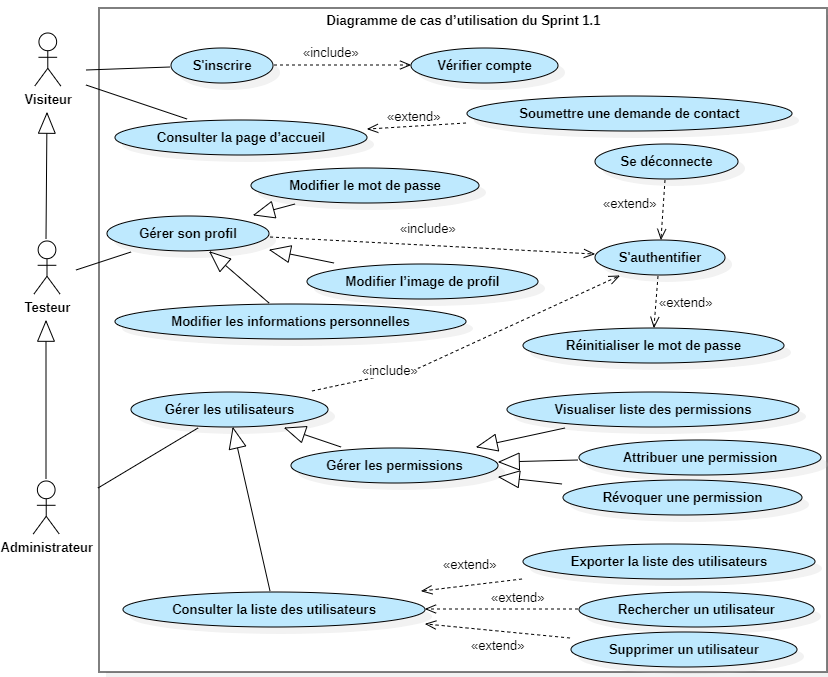
\includegraphics[width=0.92\linewidth]{chapitres/ch3Sp1/section/sprint1/img/LastUseCaseSprint1.1.png}
    \caption{Diagramme de cas d’utilisation du sprint 1.1}
    \label{fig:caseS1}
\end{figure}
\vspace{-0.5cm}
\subsubsection{Raffinement des cas d’utilisation}
Cette étape a permis de mieux comprendre les interactions, de repérer les dépendances et de découper les fonctionnalités.
\begin{enumerate}[label=\alph*), left=-0.1cm]
    \item \textbf{Raffinement du cas d’utilisation «S'inscrire»:}\\
        L'inscription inclut la saisie et validation des informations, la confirmation par e-mail avec un code OTP et la gestion des erreurs pour garantir une expérience utilisateur optimale.
        \begin{itemize}[label=\ding{111}, left=-0.1cm]
            \item \textbf{Description textuelle du cas d’utilisation "S'inscrire":} \\
                  Le tableau ~\ref{tab:descInsc}  présente la description textuelle du cas d’utilisation "S'inscrire".
                  \begin{spacing}{1.1}
                        \begin{longtable}{|p{0.12\linewidth}|p{0.88\linewidth}|}
                            \caption{Description textuelle du cas d’utilisation : S'inscrire}
                            \label{tab:descInsc}\\
                            \hline
                            \textbf{Titre} & S'inscrire \\
                            \hline
                            \textbf{Acteur} & Visiteur \\
                            \hline
                            \textbf{Résumé} & Ce cas d'utilisation décrit le processus d'inscription permettant au visiteur de créer un compte personnel. \\
                            \hline
                            \textbf{Pré-conditions} & 
                                Le visiteur doit disposer d’un accès à Internet via un dispositif connecté (ordinateur, tablette, smartphone). \\
                            \hline
                            \textbf{Post-conditions} & 
                                Un nouveau compte utilisateur est créé, et un email de confirmation contenant un code OTP est envoyé afin de vérifier l’adresse email saisie. \\
                            \hline
                            \textbf{Scénario nominal} & 
                            \begin{minipage}{\linewidth}
                                \vspace{0.1cm}
                                \begin{enumerate}[label=\arabic*., left=-0.05cm]
                                    \item Le visiteur accède à la page d'inscription et clique sur le bouton "Inscrire".
                                    \item Le système affiche un formulaire de saisie des informations d'inscription.
                                    \item Le visiteur remplit le formulaire avec ses informations, puis le soumet.
                                    \item Le système valide les informations fournies.
                                    \item Le système enregistre les données du visiteur dans la base de données.
                                    \item Il génère automatiquement des identifiants de connexion.
                                    \item Le système envoie un e-mail de confirmation contenant un code OTP (One-Time Password) de 6 chiffres.
                                    \item L'utilisateur saisit ce code dans un champ dédié.
                                    \item Une fois le code validé avec succès, l'adresse e-mail est vérifiée et l'inscription est finalisée.
                                \end{enumerate}
                                \vspace{0.05cm}
                            \end{minipage}\\
                            \hline
                            \textbf{Scénario d’erreur} &
                            \begin{minipage}{\linewidth}
                                \vspace{0.1cm}
                                \begin{itemize}[left=0cm]
                                    \item[\textbullet] \textbf{Étape 4 (Informations incomplètes):}
                                    \begin{itemize}[label=\ding{56}]
                                        \item Si des champs obligatoires sont laissés vides, le système affiche un message d’erreur précisant les champs à compléter.
                                        \item L'utilisateur est invité à fournir les informations manquantes.
                                    \end{itemize}
                        
                                    \item[\textbullet] \textbf{Étape 4 (Annulation) :}
                                    \begin{itemize}[label=\ding{56}]
                                        \item L'utilisateur peut annuler l'inscription avant la soumission. Aucun enregistrement n’est effectué.
                                    \end{itemize}
                        
                                    \item[\textbullet] \textbf{Étape 7 (Erreur d'enregistrement):}
                                    \begin{itemize}[label=\ding{56}]
                                        \item En cas d’échec lors de l’enregistrement des données, le système affiche un message d’erreur et invite à réessayer ultérieurement.
                                    \end{itemize}
                        
                                    \item[\textbullet] \textbf{Étape 9  (Expiration du code OTP) :}
                                    \begin{itemize}[label=\ding{56}]
                                        \item Le code OTP possède une durée de validité limitée. En cas de dépassement, un message informe l’utilisateur de l’expiration du code et lui propose d’en générer un nouveau via le lien contenu dans l’e-mail.
                                    \end{itemize}
                        
                                    \item[\textbullet] \textbf{Étape 10 (Code OTP incorrect):}
                                    \begin{itemize}[label=\ding{56}]
                                        \item Si l'utilisateur saisit un code OTP erroné, le système affiche un message d'erreur et l'invite à le ressaisir.
                                        \item Après plusieurs tentatives échouées, le système bloque temporairement la validation par OTP et propose l'envoi d'un nouveau code.
                                    \end{itemize}
                                \end{itemize}
                                \vspace{0.1cm}
                            \end{minipage}\\
                            \hline
                        \end{longtable}
                    \end{spacing}
                  \vspace{-0.2cm}
            \item \textbf{Diagramme  de séquence du cas d’utilisation "S'inscrire":} \\ Les étapes de déroulement du cas d’utilisation "S'inscrire" sont décrites par le diagramme de séquence illustré par la figure ~\ref{fig:seqInscrire}.
            \begin{figure}[H]
                \centering
                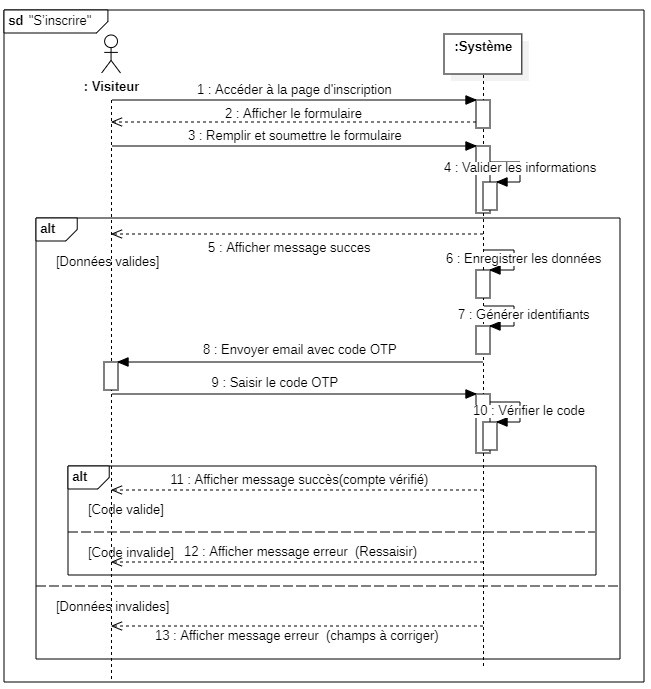
\includegraphics[width=0.9\textwidth]{chapitres/ch3Sp1/section/sprint1/img/seq-creer-compte-sp1.png}
                \caption{Diagramme de séquence du cas d’utilisation de "S'inscrire"}
                \label{fig:seqInscrire}
            \end{figure}
        \end{itemize}
    
  \item \textbf{Raffinement du cas d’utilisation « Gérer les permissions des utilisateurs » :}\\
    Cette section détaille le raffinement du cas d’utilisation « Gérer les permissions des utilisateurs ». Ce cas d’utilisation permet à un administrateur de gérer les droits d’accès des utilisateurs aux différentes permissions (fonctionnel, SEO, sécurité...).
     \begin{itemize}[label=\ding{111}, left=-0.1cm]
            \item \textbf{Description textuelle du cas d’utilisation "Attribuer des permissions" :}\\
            Le tableau \ref{tab:descAttribuerPermissions} décrit textuellement le cas d’utilisation <<Attribuer des permissions>>.
            \begin{spacing}{1.2}
                \begin{longtable}{|p{0.12\linewidth}|p{0.88\linewidth}|}
                \caption{Description textuelle du cas d’utilisation : Attribuer des permissions}
                \label{tab:descAttribuerPermissions} \\
                \hline
                \textbf{Titre} & Attribuer des permissions \\
                \hline
                \textbf{Acteur} & Administrateur \\
                \hline
                \textbf{Résumé} & Ce cas d'utilisation permet à l’administrateur d’attribuer à un utilisateur des permissions d’accès aux tests (fonctionnel, SEO, sécurité). \\
                \hline
                \textbf{Pré-conditions} & L’utilisateur concerné doit exister dans le système. L’administrateur doit être connecté. \\
                \hline
                \textbf{Post-conditions} & Les permissions sélectionnées sont enregistrées et appliquées à l’utilisateur dans la base de données. \\
                \hline
                \textbf{Scénario nominal} &
                \begin{minipage}{\linewidth}
                \vspace{0.1cm}
                \begin{enumerate}[label=\arabic*., left=0.2cm]
                    \item L’administrateur accède à l’interface de gestion des permissions.
                    \item Il sélectionne un utilisateur.
                    \item Il choisit les permissions à autoriser.
                    \item Il valide la configuration.
                    \item Le système enregistre les nouvelles permissions.
                \end{enumerate}
                \vspace{0.1cm}
                \end{minipage} \\
                \hline
                \textbf{Scénario d’erreur} &
                \begin{minipage}{\linewidth}
                    \vspace{0.1cm}
                    \begin{itemize}[left=0cm]
                        \item[\textbullet] \textbf{Erreur d’enregistrement :} En cas d’échec d’écriture en base de données, le système signale une erreur et annule l’opération.
                    \end{itemize}
                    \vspace{0.1cm}
                \end{minipage} \\
                \hline
                \end{longtable}
            \end{spacing}
            \vspace{-0.2cm}
            \item  \textbf{Diagramme d’activité : Vérification des permissions d’accès:}\\
                Le diagramme d’activité de la figure \ref{fig:permission-activite} illustre le processus de gestion conditionnelle des droits d’accès. Après l’authentification, le système accorde aux administrateurs un accès complet leur permettant d’attribuer des permissions.
            \begin{figure}[H]
        \centering
        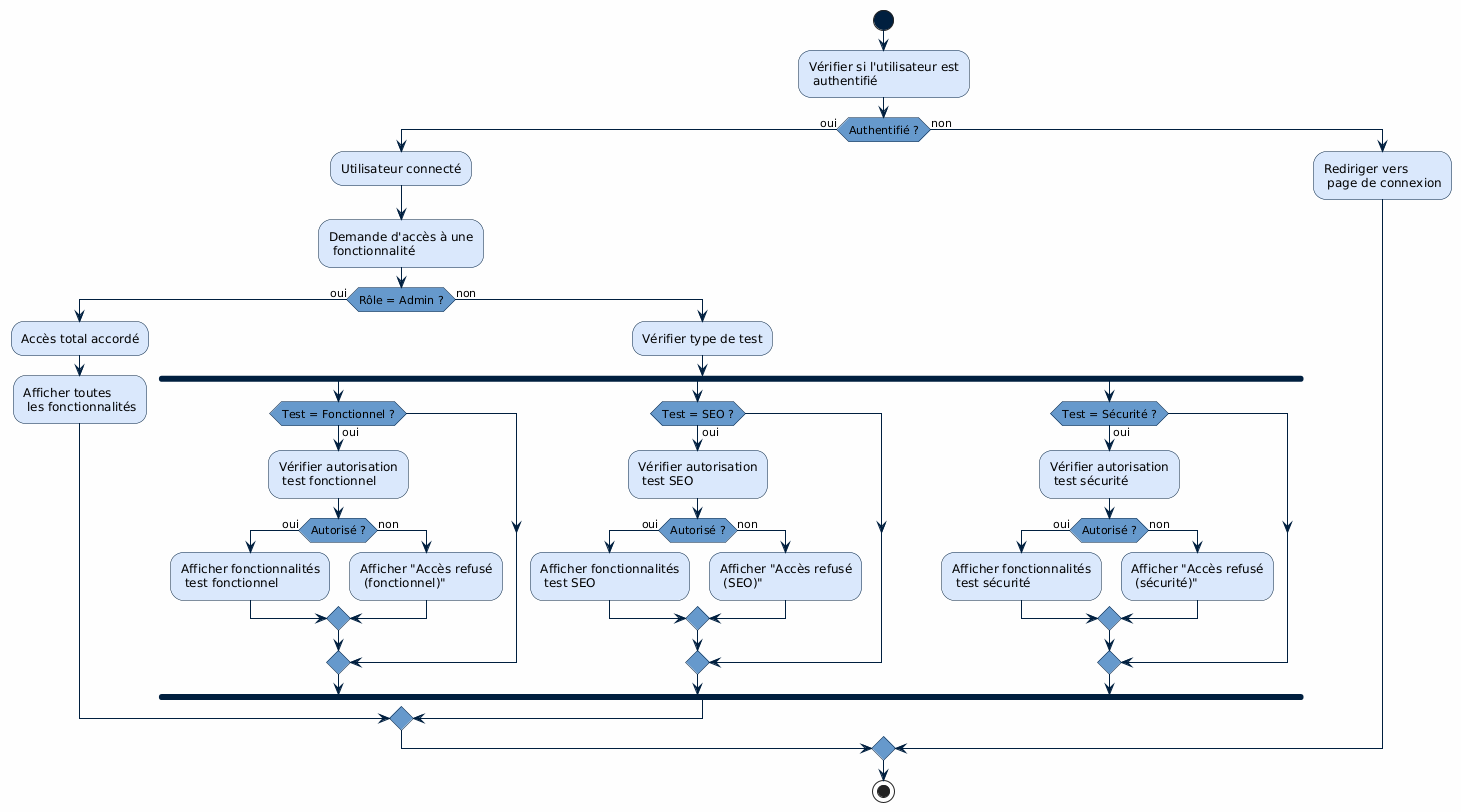
\includegraphics[width=\linewidth]{chapitres/ch3Sp1/section/sprint1/img/permission-activite.png}
        \caption{\centering Diagramme d’activité : Processus de vérification des permissions lors de la demande d’accès à une fonctionnalité}
        \label{fig:permission-activite}
    \end{figure}
    \end{itemize}
    \vspace{-0.5cm}
\end{enumerate}